\section{Experiments}\label{sec:exp}

% Table generated by Excel2LaTeX from sheet 'ram config'
\begin{table*}[htbp]
  \centering
  \caption{Device parameters used for I/O buffer, weight buffer and DDR.}
  \vspace{-5pt}
    \begin{tabular}{|r|r|r|r|r|r|r|r|r|}
    \hline
          & bitwidth (B) & size (B) & Rd BW (GB/s) & Wr BW (GB/s) & Rd Ene (pJ) & Wr Ene(pJ) & Leakage (mW) & Area ($um^2$)\\
    \hline
    \multicolumn{1}{|c|}{} & 32    & 128K  & 15.169  & 1.556  & 67.690  & 195.286  & 0.04000  & 21224 \\
\cline{2-9}    \multicolumn{1}{|c|}{22nm} & 32    & 256K  & 11.693  & 1.534  & 75.071  & 217.468  & 0.04104  & 26707 \\
\cline{2-9}    \multicolumn{1}{|c|}{LSTP} & 32    & 512K  & 8.005  & 1.490  & 88.483  & 260.073  & 0.04314  & 37308\\
\cline{2-9}    \multicolumn{1}{|c|}{RRAM} & 32    & 1M    & 11.056  & 1.534  & 133.189  & 268.319  & 0.05282  & 61090 \\
\cline{2-9}    \multicolumn{1}{|c|}{} & 32    & 2M    & 10.306  & 1.534  & 231.750  & 357.190  & 0.07806  & 107007 \\
    \hline
    \multicolumn{1}{|c|}{} & 8     & 16K   & 9.145  & 5.147  & 3.057  & 0.556  & 0.00134  & 10031 \\
\cline{2-9}    \multicolumn{1}{|c|}{22nm} & 8     & 32K   & 8.609  & 4.973  & 6.432  & 1.315  & 0.00270  & 20048 \\
\cline{2-9}    \multicolumn{1}{|c|}{LSTP} & 8     & 64K   & 16.831  & 11.763  & 6.780  & 3.777  & 0.00600  & 42803 \\
\cline{2-9}    \multicolumn{1}{|c|}{SRAM} & 8     & 128K  & 10.977  & 10.451  & 7.931  & 2.792  & 0.01153  & 82032 \\
\cline{2-9}    \multicolumn{1}{|c|}{} & 8     & 256K  & 10.977  & 10.451  & 11.562  & 6.424  & 0.02306  & 164065 \\
    \hline
    \multicolumn{1}{|c|}{DDR4} & 4    & 128M  & \multicolumn{2}{c|}{3.2} & 80.300  & 82.719  & 52.80000  & N/A \\
    \hline
    \end{tabular}%
  \label{tab:device}%
\end{table*}%

Experiments are carried out on the architecture introduced in Section~\ref{sec:hw}, with the scheduling strategy in section~\ref{sec:schedule} applied. We use a behavior level simulator to analyze the memory access and computation energy for running a certain network. Memory access dynamic energy cost, memory static energy cost and computation energy cost are considered in our model.

\subsection{Experiment setup}
The MAC array in the architecture is configured as an $8\times8\times8$ array running at 1GHz. This offers a peak performance of 1TOP/s. 8-bit multiplication and 32-bit accumulation are adopted in this model. Multiplication and addition energy is scaled down from the data in~\cite{mac_energy} to 22nm technology. 

The above configuration requires the read bandwidth of input/output buffer and weight buffer to be at least 64GB/s. We implement each buffer with 8 banks and each of them should offer 8GB/s read bandwidth. On-chip memory parameters are generated from NVSim~\cite{dong2014nvsim} with different memory size configurations. RRAM buffer bit width is configured as 256bit to achieve enough bandwidth. 

The external memory parameter is generated from MICRON DDR4 power calculator~\cite{powercalc}. The generated dynamic I/O power is further converted to energy per read or write byte. In our experiment, we use 2 DDR chips as external memory because the bandwidth can support the configured MAC array with proposed schedule strategy and the size is enough. To reduce background power overhead, we use the least number of chips. All the detailed data and configuration is shown in Table~\ref{tab:device}. 

The buffer in the accumulator is also considered in our experiments. 4 types of buffers are chosen for design space exploration. Corresponding parameters are generated by NVSim and are shown in Table~\ref{tab:small_buf}.

\begin{table}[htbp]
  \centering
  \caption{32-bit accumulation buffer parameters.}
  \vspace{-5pt}
    \begin{tabular}{|r|r|r|r|r|}
    \hline
    depth & 16    & 32    & 64    & 128 \\
    \hline
    energy per read (pJ) & 0.045 & 0.056 & 0.107 & 0.12 \\
    \hline
    energy per write (pJ) & 0.022 & 0.031 & 0.083 & 0.094 \\
    \hline
    area ($um^2$) & 57.673 & 103.422 & 188.714 & 354.138 \\
    \hline
    Leakage (nW) & 6.162 & 11.133 & 22.385 & 44.823 \\
    \hline
    \end{tabular}%
  \label{tab:small_buf}%
\end{table}%

\subsection{Energy Cost Analysis}
We do experiments on all the combinations of the RAM configurations in Table \ref{tab:device} and \ref{tab:small_buf}, which means $5\times 5\times 5 = 125$ choices for an SRAM or RRAM based accelerator. The three schedule strategies in section~\ref{sec:schedule} is applied to each choice. Figure~\ref{fig:design_space} shows the experimental result with the convolution layers of VGG-11 network for 1 input. The energy cost of computation and DDR leakage is marked and is the same for all the designs because the network is fixed and all the designs are computation bounded. So the processing time is a constant to all the designs. In general, the RRAM based design consumes less energy compared with an SRAM design of the same area. The minimal energy design for SRAM and RRAM costs 3086uJ and 2532uJ respectively, meaning that using RRAM can save 18\% system energy. The RRAM design is also 15\% smaller than the SRAM design. We also do experiments with the convolution layers of VGG-16 and AlexNet, where RRAM design saves 18\% and 12\% energy with 15\% and 75\% less on-chip RAM area compared with SRAM design.

\begin{figure*}[t]
  \centering
  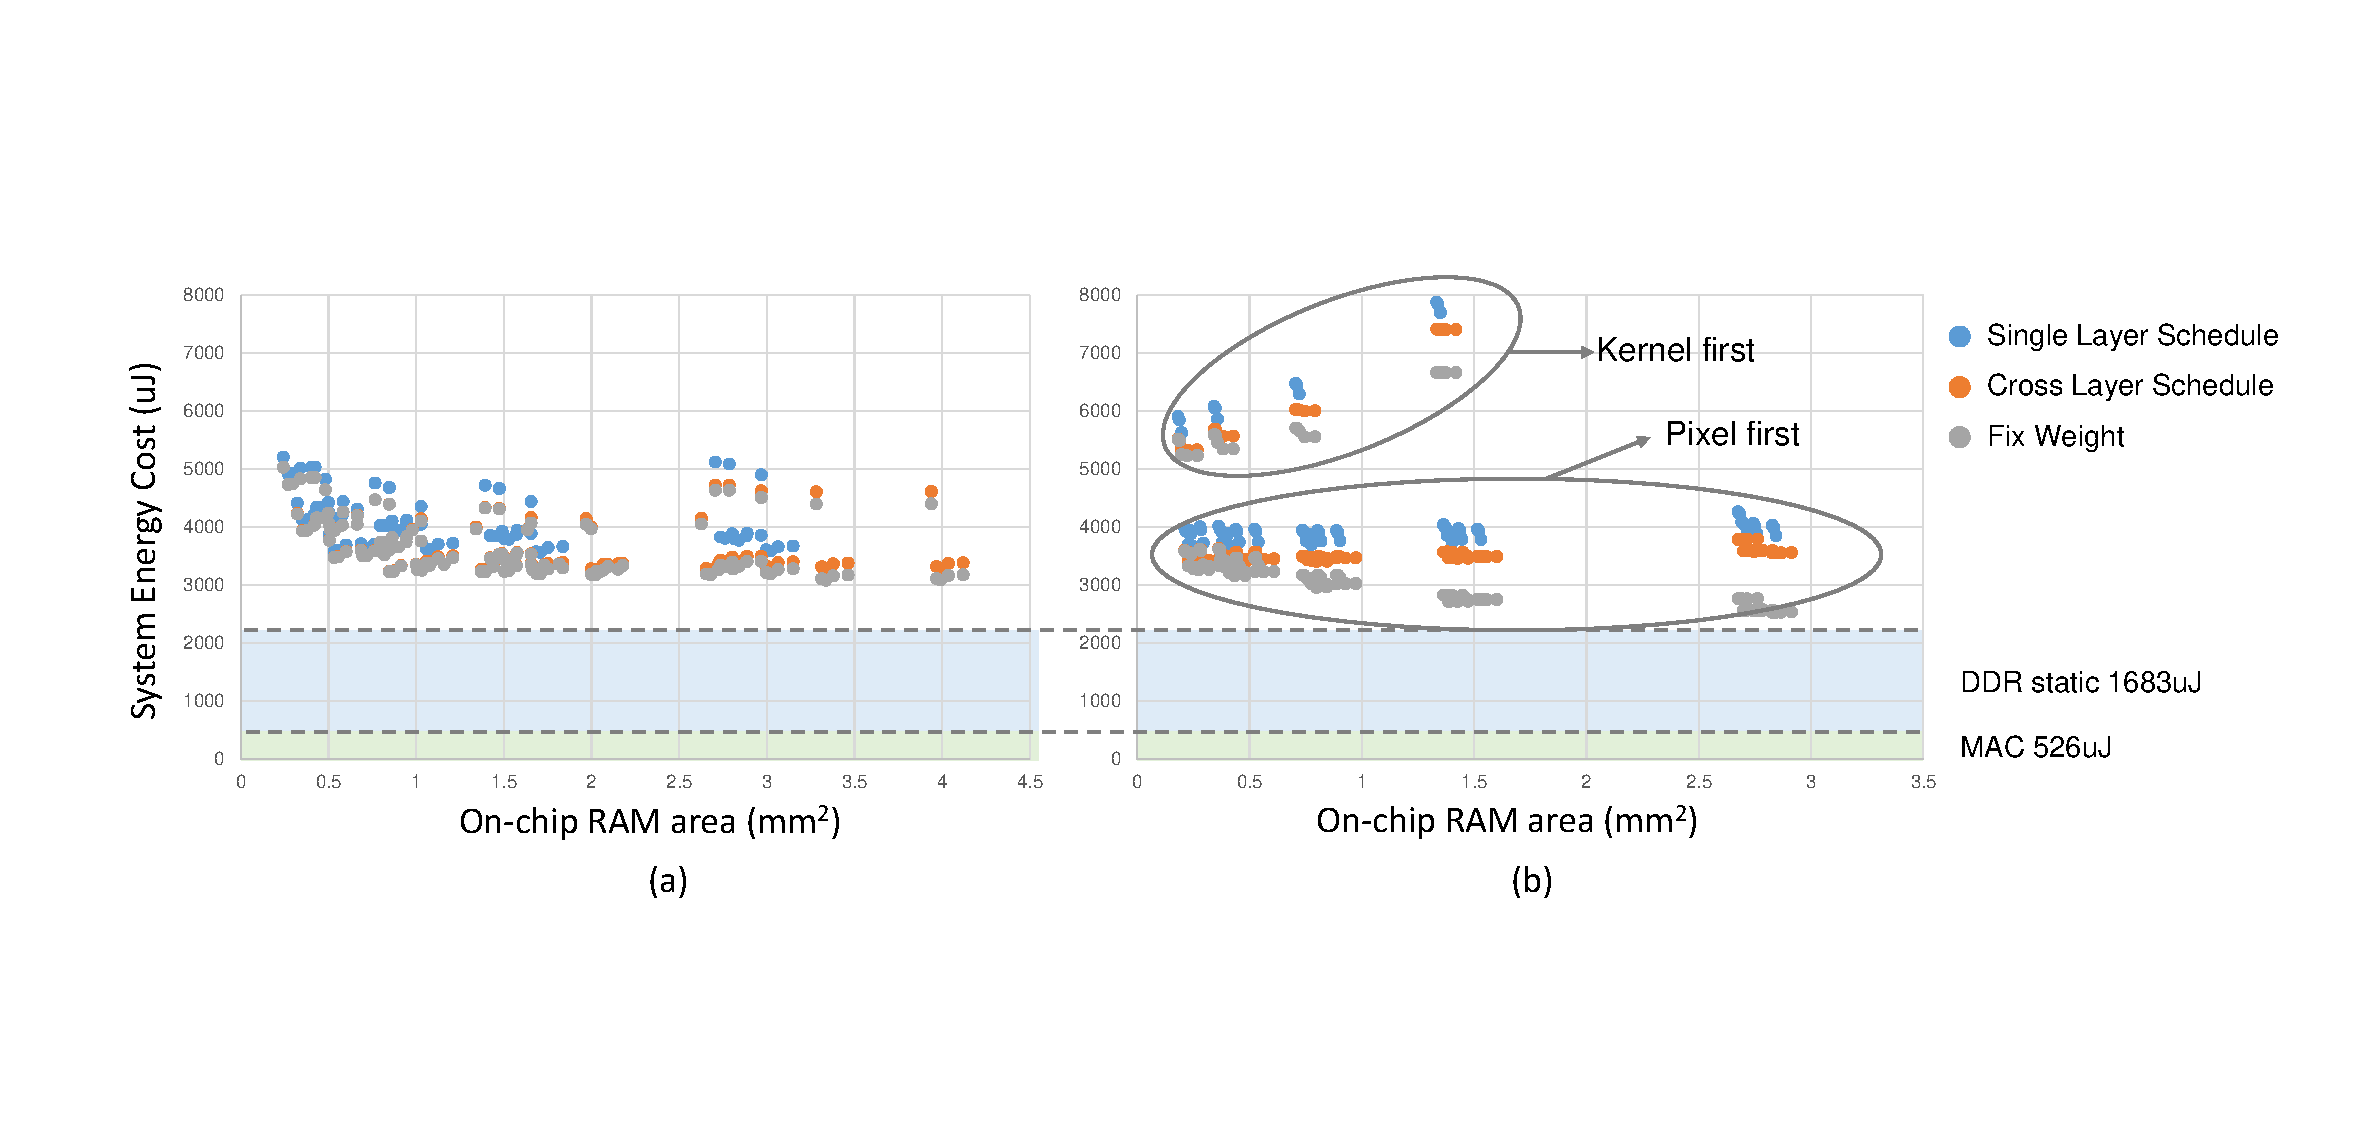
\includegraphics[width=2\columnwidth]{fig/design_space.pdf}
  \vspace{-10pt}
  \caption{Design space exploration on different hardware choices and schedule strategies on the convolution layers of VGG-11 model. (a) SRAM weight buffer design. (b)RRAM weight buffer design.}
  \label{fig:design_space}
  \vspace{-5pt}
\end{figure*}

We examine the effect of the proposed hardware optimization and scheduling strategy. First, the loop order is the key effect to the RRAM based design, as shown in Figure~\ref{fig:design_space}(b). Note that some of the design points with the kernel first loop order are out of the figure because the energy cost is larger than 8000uJ. The large read energy of RRAM dominates the system energy as the capacity of RRAM increases. The reduction in DDR access cannot compensate for this overhead. Even on the smallest design, changing the loop order to pixel first will save at least 1/3 of the system energy cost. 

A breakdown of the on-chip buffer energy cost is shown in Figure~\ref{fig:breakdown}(a). The largest designs, in our experiment the designs with 4MB SRAM input/output buffer and 2MB SRAM (or 16MB RRAM) weight buffer are used. Here we only consider the read energy of input/output buffer and weight buffer and the dynamic energy of accumulation buffer. The write energy to input/output buffer and leakage energy are not affected by the accumulation buffer and thus not considered. Up to $96\%$ energy is saved for the RRAM based designs consider the overhead brought by the accumulation buffer. SRAM design also benefits from the change in loop order but not as effective as to the RRAM designs.

\begin{figure*}[t]
  \centering
  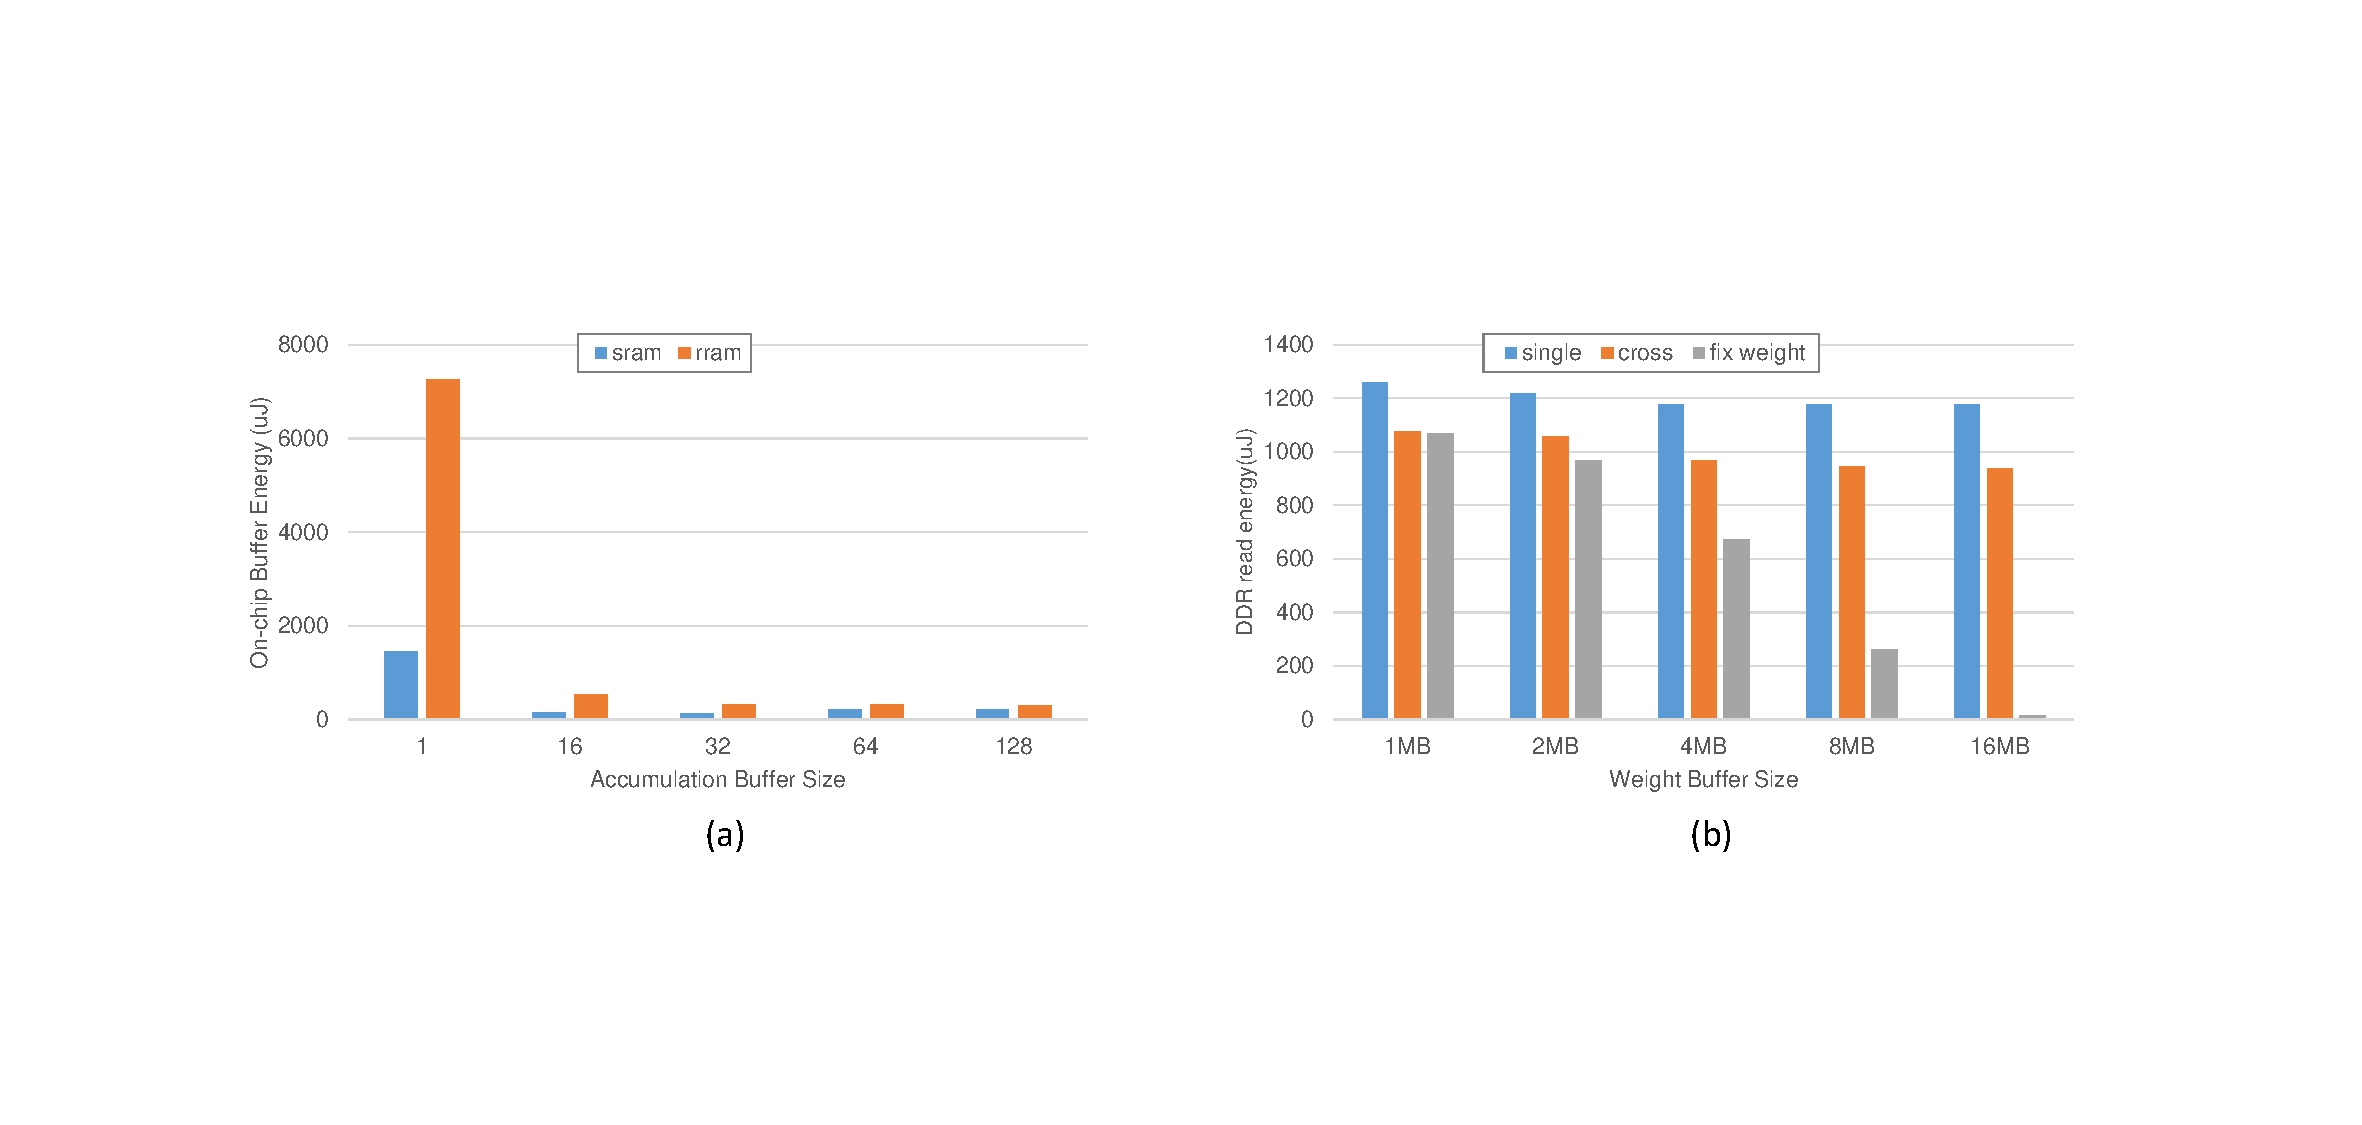
\includegraphics[width=1.8\columnwidth]{fig/breakdown.pdf}
  \vspace{-10pt}
  \caption{(a) On-chip buffer energy cost for a series of designs only differs in accumulation buffer size. (b) DDR access energy cost for a series of designs only differs in weight buffer size.}
  \label{fig:breakdown}
  \vspace{-15pt}
\end{figure*}

Second, fixing the weight on-chip helps the hardware fully utilize the on-chip RAM to reduce off-chip data transfer. As can be seen from Figure~\ref{fig:design_space}(b), using the pixel first loop order, the accelerator cannot benefit from a larger on-chip buffer with single-layer scheduling and cross-layer scheduling. By fixing some of the network weights on-chip, the system energy cost is gradually reduced as the on-chip RAM size increases. 

A breakdown of the DDR transfer cost is shown in Figure~\ref{fig:breakdown}(b). All the designs implement no accumulation buffer and 1MB SRAM as input/output buffer. The single layer scheduling and cross-layer scheduling can only achieve $6.4\%$ and $13.5\%$ energy saving respectively when the weight buffer increases from 1MB to 16MB. With the fix weight strategy, the energy saving is $98.5\%$. 